\begin{figure}[H]
    % ROW 1
    
    \begin{subfigure}[t]{.24\textwidth}
        \begin{subfigure}[t]{\textwidth}
            \caption{}
            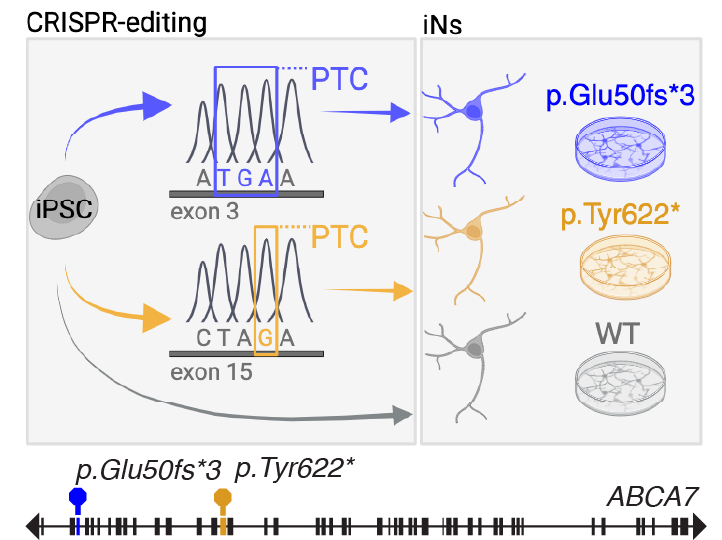
\includegraphics[width=\textwidth]{./main_plots/iN_cartoon.png}        
        \end{subfigure} 
        \begin{subfigure}[t]{\textwidth}
            \caption{}
            \includegraphics[width=\textwidth]{./extended_plots/rna_correlation_both_lof_lines.png}        
        \end{subfigure} 
    \end{subfigure} 
    \hspace{.5cm}
    \begin{subfigure}[t]{.23\textwidth}
        \begin{subfigure}[t]{\textwidth}
            \caption{}
            \includegraphics[width=\textwidth]{./main_plots/y622_kl_clusters_network.pdf}        
        \end{subfigure}
        \begin{subfigure}[t]{\textwidth}
            \caption{}
            \centering
            \includegraphics[width=0.5\textwidth]{./main_plots/jaccard_cartoon.png}        
            \includegraphics[width=\textwidth]{./main_plots/jaccard_PM_pT622.png}        
        \end{subfigure}  
    \end{subfigure} 
    \hspace{.25cm}
    \begin{subfigure}[t]{.45\textwidth}
        \caption{}
        \includegraphics[width=\textwidth]{./main_plots/kl_densities_Tyr622.png}        
    \end{subfigure}  
    % Row 2
    \vspace{.25cm}
    \begin{subfigure}[t]{.25\textwidth}
        \begin{subfigure}[t]{\textwidth}
            \caption{}
            \includegraphics[width=\textwidth]{./main_plots/y622_mito_degs.png}        
        \end{subfigure}  
    \end{subfigure} 
    \begin{subfigure}[t]{.2\textwidth}
        \caption{}
            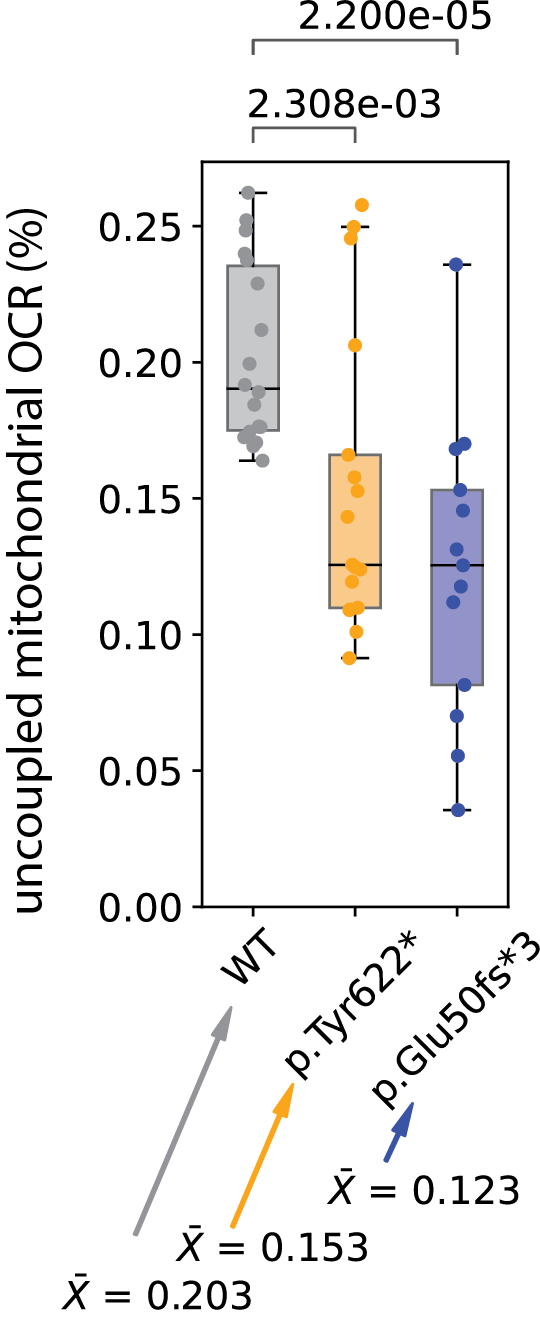
\includegraphics[width=\textwidth]{./main_plots/uncoupling.png}        
    \end{subfigure}   
    \begin{subfigure}[t]{.45\textwidth}
        \caption{}
        \includegraphics[width=\textwidth]{./extended_plots/mitohealth_y_g.png}        
    \end{subfigure}    
    % Row 3
    \begin{subfigure}[t]{.35\textwidth}
        \caption{}
        \includegraphics[width=\textwidth]{./main_plots/tmrm_main.png}        %tmrm_with_FCCP
    \end{subfigure}    
   % \hspace{1cm}
    \hspace{.25cm}
    \begin{subfigure}[t]{.35\textwidth}
        \caption{}
        \includegraphics[width=\textwidth]{./main_plots/cellrox_images.png}        
    \end{subfigure}  
    \hspace{.5cm}
    \begin{subfigure}[t]{.25\textwidth}
        \caption{}
        \includegraphics[width=\textwidth]{./main_plots/all_lipids_y622.png}        
    \end{subfigure}  
    \caption{
        \textbf{ABCA7 LoF Impairs Regulation of Mitochondrial Uncoupling in Neurons.}\\
    }
    \label{fig:main_mitochondrial}
\end{figure}
\begin{itemize}
\item[\textbf{(A)}] Schematic of iPSC-derived isogenic neuronal lines carrying ABCA7 LoF variants. The ABCA7 gene map highlights exons (black rectangles) and introns (black lines). CRISPR-Cas9 was used to introduce a premature termination codon in exon 3 (p.Glu50fs3, blue) or exon 15 (p.Tyr622, orange).\\
\item[\textbf{(B)}] Correlation of per-gene perturbation scores ($S = -\log_{10}(\text{p-value}) \times \text{sign}(\log_2(\text{fold change}))$) between p.Glu50fs3 vs. WT and p.Tyr622 vs. WT iNs.\\
\item[\textbf{(C)}] Kernighan-Lin (K/L) clustering of leading-edge genes from pathways perturbed in p.Tyr622* vs. WT iNs (p-adjusted < 0.05). Colors indicate distinct K/L gene clusters, which are assigned postmortem (PM) cluster labels if they significantly overlap with PM-identified clusters based on Jaccard analysis in (D). Otherwise, they are labeled with a 'T' prefix.\\
\item[\textbf{(D)}] Heatmap showing Jaccard index-based overlap between K/L clusters from p.Tyr622* vs. WT iNs and postmortem-identified clusters.\\
\item[\textbf{(E)}] Left: Gaussian kernel density estimate plots of gene scores $S$ for genes within each cluster ($S>0$ indicates upregulation in ABCA7 LoF). Solid lines represent distribution means. Right: Top representative pathways associated with the highest intra-cluster connectivity.\\
\item[\textbf{(F)}] Volcano plot of differentially expressed genes between p.Tyr622* and WT iNs, highlighting genes with mitochondrial localization.\\
\item[\textbf{(G)}] Uncoupled mitochondrial oxygen consumption rate (OCR) in WT vs. ABCA7 LoF iNs, measured by Seahorse assay. P-values computed via independent sample t-test. $N$ wells = 18 (WT), 17 (p.Tyr622*), 13 (p.Glu50fs*3) from two independent differentiation batches.\\
\item[\textbf{(H)}] Left: Quantification of mitochondrial membrane potential using HCS MitoHealth dye in neurons. P-values computed using a linear mixed-effects model on per-NeuN+ volume averages, with well-of-origin as a random effect. $N=8$ (WT), 11 (p.Tyr622*), 9 (p.Glu50fs*3), with ~3000 cells per condition from three independent differentiation batches. Right: Representative images showing NeuN+ cells and corresponding MitoHealth and Hoechst staining. MitoHealth images underwent percentile-based background subtraction and thresholding.\\
\item[\textbf{(I)}] Average TMRM fluorescence intensity in p.Tyr622* vs. WT iNs per mask (binarized TMRM signal based on the 75th percentile threshold) under baseline conditions and after FCCP treatment.\\
\item[\textbf{(J)}] Average CellROX fluorescence intensity in p.Tyr622* vs. WT iNs per mask (binarized CellROX signal based on the 75th percentile threshold).\\
\item[\textbf{(K)}] Volcano plot of differentially abundant lipid species between p.Tyr622* and WT iNs, colored by lipid class.
\end{itemize}